\scanpage{72}\mspage{71}

Pour la suite, il faut faire attention si les axiomes vont passer aux sous-contrées. Introduisons quand $= =$ la définition en forme

% fig-definition: the raised word and its full hooked connector, with adjoining text once.
\figure{\begin{tikzpicture}[x=1cm,y=1cm]
\node[anchor=west] at (0,0) {\uline{Définition 1} On appelle};
\node[anchor=west] at (7.4,0) {\uline{sous-contrée}};
\node[anchor=west] at (9.4,0.8) {\inserted{[\uline{pleine}]}};
\draw[line width=.55pt] (8.45,.48) .. controls (8.0,.28) and (10.9,.22) .. (11.35,.1) .. controls (11.85,.02) and (11.9,-.12) .. (12.0,-.23) .. controls (12.17,.03) and (12.28,.37) .. (12.31,.55);
\node[anchor=west] at (0,-1.05) {de la contrée $\unsure{\rlap{$\deleted{\mathcal F}$}\mathcal C|\mathcal C|\mathscr C|\mathbb C}=(\mathcal F,\leq,\preceq)$, \unsure{tout|\deleted{tout}}};
\node[anchor=west] at (0,-1.85) {sous-ens. qui \unsure{satisfont|satisfait} les conditions};
\end{tikzpicture}}

% fig-a-insertions: correspond joins the physical line-end hyphen under convention 7; both insertion arms remain.
\figure{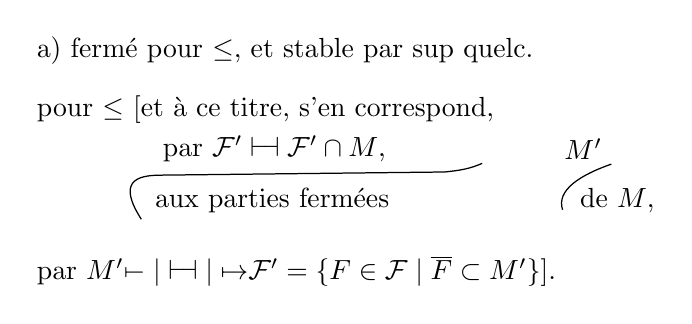
\begin{tikzpicture}[x=1cm,y=1cm]
\node[anchor=west] at (0,0) {a) fermé pour $\leq$, et stable par sup quelc.};
\node[anchor=west] at (0,-.75) {pour $\leq$ [et à ce titre, s'en correspond,};
\node[anchor=west] at (1.5,-1.9) {aux parties fermées};
\node[anchor=west] at (6.9,-1.9) {de $M$,};
\node[anchor=west] at (1.6,-1.25) {\inserted{par $\mathcal F'\mathrel{\vdash\joinrel\dashv}\mathcal F'\cap M$,}};
\node[anchor=west] at (6.7,-1.25) {\inserted{$M'$}};
\draw[line width=.45pt] (1.45,-2.14) .. controls (1.15,-1.67) and (1.37,-1.58) .. (1.7,-1.58) -- (5.3,-1.54) .. controls (5.5,-1.52) and (5.62,-1.50) .. (5.78,-1.43);
\draw[line width=.45pt] (6.8,-2.02) .. controls (6.72,-1.77) and (7.02,-1.58) .. (7.42,-1.44);
\node[anchor=west] at (0,-2.8) {par $M'\unsure{\mathrel{\mapstochar\relbar}|\mathrel{\vdash\joinrel\dashv}|\mapsto}\mathcal F'=\{F\in\mathcal F\mid\overline F\subset M'\}$].};
\end{tikzpicture}}

% slanted left margin; the terminal close is covered by root crop a05.
\margin{Je ne sais s'il faut prendre des sup quelconques (\unsure{condition} stricte) \deleted{\unsure{et}} ou bien de sup finis seulement \unsure{(condition lge)|(condition large)}}

% fig-b-correction: replacement above the cancelled clause; crossed/curling mark after M.
\figure{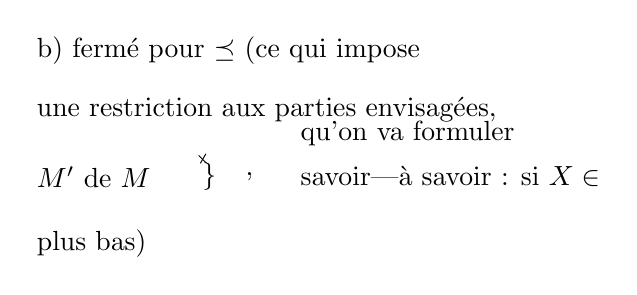
\begin{tikzpicture}[x=1cm,y=1cm]
\node[anchor=west] at (0,0) {b) fermé pour $\preceq$ (ce qui impose};
\node[anchor=west] at (0,-.75) {une restriction aux parties envisagées,};
\node[anchor=west] at (0,-1.6) {$M'$ de $M$};
% fig-b-curled-mark: curled stroke with a small crossing at its head.
\node[anchor=west] at (2.1,-1.6) {\unsure{\}}};
\draw[line width=.35pt] (2.18,-1.33) -- (2.28,-1.43);
\draw[line width=.35pt] (2.20,-1.43) -- (2.27,-1.31);
\node[anchor=west] at (2.65,-1.6) {,};
\node[anchor=west] at (3.35,-1.6) {\deleted{\unsure{savoir|à savoir} : si $X\in$}};
\node[anchor=west] at (3.35,-1.05) {\inserted{qu'on va formuler}};
\node[anchor=west] at (0,-2.45) {plus bas)};
\end{tikzpicture}}

% fig-marginal-c: marginal continuation above C6; labels occur only here.
\figure{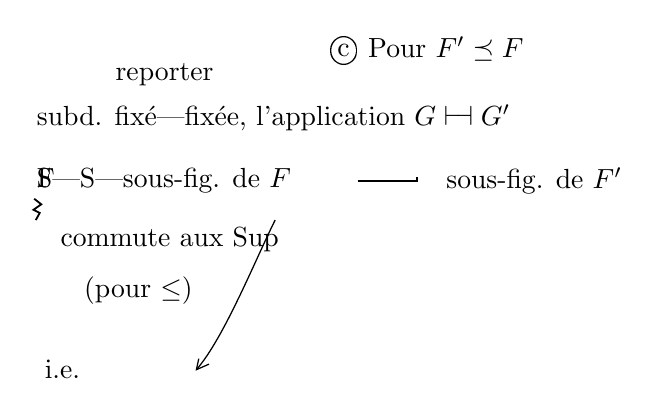
\begin{tikzpicture}[x=1cm,y=1cm]
\node[anchor=west] at (1.0,.55) {reporter};
\node[anchor=west] at (3.7,.85) {\textcircled{c} Pour $F'\preceq F$};
\node[anchor=west] at (0,0) {subd. \unsure{fixé|fixée}, l'application $G\mathrel{\vdash\joinrel\dashv}G'$};
% The worked initial is ONE letter position, including the lower residual strokes.
\node[anchor=west] at (0,-.8) {\unsure{\rlap{\deleted{F}}S|S|s}ous-fig. de $F$};
\draw[line width=.65pt] (.09,-1.03) -- (.18,-1.10) -- (.08,-1.17) -- (.16,-1.21) -- (.11,-1.30);
% fig-c-headless-link: horizontal stroke with a very short raised right endpoint, no arrowhead.
\draw[line width=.6pt] (4.2,-.8) -- (4.95,-.8) -- (4.95,-.75);
\node[anchor=west] at (5.2,-.8) {sous-fig. de $F'$};
\node[anchor=west] at (.3,-1.55) {commute aux Sup};
\node[anchor=west] at (.6,-2.2) {(pour $\leq$)};
\node[anchor=west] at (.1,-3.2) {i.e.};
% A distinct pointer descends leftward from the aux region.
\draw[line width=.45pt] (3.15,-1.3) .. controls (2.9,-1.8) and (2.5,-2.8) .. (2.15,-3.2);
\draw[line width=.45pt] (2.18,-3.06) -- (2.15,-3.2) -- (2.31,-3.13);
\end{tikzpicture}}

% diagram: C6-group. Diagrams remain diagrams; the two side rules, detached
% points and oblique gloss keep their relative positions. No text is repeated.
\diagram{\begin{tikzpicture}[x=1cm,y=1cm]
\node[anchor=west] at (0,0) {\uline{C6}};
\node[anchor=west] at (2.15,0) {Soit};
\node at (4.05,-1.45) {\begin{tikzcd}[ampersand replacement=\&,column sep=1.6em,row sep=1.5em]
F' \arrow[r,phantom,"{\preceq}" description] \& F \arrow[d,phantom,"{\rotatebox{90}{$\leq$}}" description] \\
\& G
\end{tikzcd}};
\node[anchor=west] at (7.90,-1.15) {de $\mathcal F$};
\fill (2.01,-.88) circle (.012);
\fill (2.08,-.93) circle (.012);
\draw[line width=.4pt] (-.30,-.18) .. controls (-.27,-1.92) and (-.34,-3.62) .. (-.19,-4.78);
% slanted; the long rule is not treated as cancellation of this gloss.
\node[anchor=west,rotate=44,align=left] at (-2.00,-2.25) {sym\unsure{e|é}trique\\en $\leq,\preceq$};
\fill (-.46,-2.12) circle (.012);
\node[anchor=west] at (0,-3.05) {\textcircled{a} Alors il existe un unique $H\in\mathcal F$ \unsure{avec|ou}};
\node at (4.10,-4.86) {\begin{tikzcd}[ampersand replacement=\&,column sep=1.6em,row sep=1.5em]
F' \arrow[r,phantom,"{\preceq}" description] \arrow[d,phantom,"{\rotatebox{90}{$\leq$}}" description] \& F \arrow[d,phantom,"{\rotatebox{90}{$\leq$}}" description] \\
G' \arrow[r,phantom,"{\preceq}" description] \& G
\end{tikzcd}};
\node[anchor=west] at (7.05,-3.73) {et};
\node at (7.72,-3.42) {\textcircled{b}};
\node[anchor=west] at (8.04,-3.73) {les \unsure{str.tes|strates} de};
\node[anchor=west] at (7.05,-4.24) {$G'$ sont les \unsure{\deleted{S}|S|s}tr\unsure{a|.}tes};
\node[anchor=west] at (7.05,-4.75) {$X'$ de $F'$ \unsure{tel|\deleted{tel}}les que};
\node[anchor=west] at (7.38,-5.25) {$X'\ll\unsure{G_n|G_m|G}$.};
\node[anchor=west] at (7.28,-5.72) {Ce compl\unsure{\.{e}|é|e}ment servira};
\node[anchor=west] at (7.48,-6.08) {plus bas};
\draw[line width=.5pt] (6.88,-3.67) -- (6.92,-5.70);
\draw[line width=.5pt] (6.98,-3.64) -- (7.02,-5.77);
\draw[line width=.45pt] (6.87,-5.39) -- (7.02,-5.72);
\draw[line width=.45pt] (6.88,-5.49) -- (7.06,-5.47);
\end{tikzpicture}}

On dit que $\unsure{G|\rlap{$\deleted{F}$}G|E}'$ est la \uline{subd} \uline{de} $G$ induite
% figure: bottom-punctuation. The slant, loop and second small curve following
% F are preserved without deciding that they are one or two commas.
\figure{\begin{tikzpicture}[x=1cm,y=1cm]
\node[anchor=west] at (0,0) {par la subd $F'$ de $F$};
\node[anchor=west] at (4.08,.02) {\unsure{\begin{tikzpicture}[x=1cm,y=1cm,baseline=-.1cm]
\draw[line width=.4pt] (.21,.30) -- (.01,-.26) .. controls (-.04,-.42) and (.11,-.42) .. (.10,-.28) .. controls (.06,-.20) and (-.01,-.22) .. (.01,-.26);
\draw[line width=.4pt] (.29,-.24) .. controls (.29,-.34) and (.23,-.39) .. (.18,-.42);
\end{tikzpicture}}};
\node[anchor=west] at (4.75,0) {ou que $G'$ est la \deleted{\unsure{sous-fig|sous-fig.}}};
\end{tikzpicture}}
% slanted
\margin{sur la sous-figure $\unsure{\rlap{$\deleted{F}$}G|G|E}$ de $F$}
